\documentclass[border=4mm]{standalone}
\usepackage{pgfplots}
\usepackage{bm}
\usepackage{xcolor}
\pgfplotsset{compat=1.12}

\definecolor{purple}{HTML}{3B3B98}
\definecolor{red}{HTML}{EA2027}
\definecolor{blue}{HTML}{0652DD}
\definecolor{green}{HTML}{26DE81}
\begin{document}
  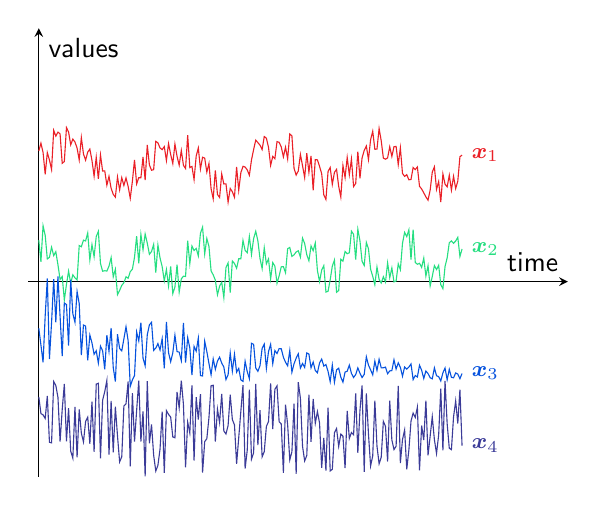
\begin{tikzpicture}
    \begin{axis}[
     axis lines=middle,clip=false,
            xmin=-0.1,xmax=5,ymin=-1,ymax=1.3,
            ytick={0},
            xtick={0},
            xlabel=$\mathsf{time}$,
            ylabel=$\mathsf{values}$]
          \addplot[domain=0:4,samples=200,red]{0.2*rnd + 0.5 + 0.1*sin(deg(2*pi*x))}
                                node[right,pos=1,font=\footnotesize]{$\bm{x}_1$};
      \addplot[domain=0:4,samples=200,green]{0.2*rnd + 0.1*cos(deg(4*pi*x))}
                                node[right,pos=1,font=\footnotesize]{$\bm{x}_2$};
      \addplot[domain=0:4,samples=200,blue]{(0.5*rnd + 0.1*sin(deg(2*pi*x)))*exp(-0.5*abs(x)) - 0.5}
                                node[right,pos=1,font=\footnotesize]{$\bm{x}_3$};
      \addplot[domain=0:4,samples=200,purple]{0.5*rnd - 1}
                                node[right,pos=1,font=\footnotesize]{$\bm{x}_4$};
    \end{axis}
  \end{tikzpicture}
\end{document}
